% Options for packages loaded elsewhere
\PassOptionsToPackage{unicode}{hyperref}
\PassOptionsToPackage{hyphens}{url}
%
\documentclass[
]{article}
\usepackage{lmodern}
\usepackage{amsmath}
\usepackage{ifxetex,ifluatex}
\ifnum 0\ifxetex 1\fi\ifluatex 1\fi=0 % if pdftex
  \usepackage[T1]{fontenc}
  \usepackage[utf8]{inputenc}
  \usepackage{textcomp} % provide euro and other symbols
  \usepackage{amssymb}
\else % if luatex or xetex
  \usepackage{unicode-math}
  \defaultfontfeatures{Scale=MatchLowercase}
  \defaultfontfeatures[\rmfamily]{Ligatures=TeX,Scale=1}
\fi
% Use upquote if available, for straight quotes in verbatim environments
\IfFileExists{upquote.sty}{\usepackage{upquote}}{}
\IfFileExists{microtype.sty}{% use microtype if available
  \usepackage[]{microtype}
  \UseMicrotypeSet[protrusion]{basicmath} % disable protrusion for tt fonts
}{}
\makeatletter
\@ifundefined{KOMAClassName}{% if non-KOMA class
  \IfFileExists{parskip.sty}{%
    \usepackage{parskip}
  }{% else
    \setlength{\parindent}{0pt}
    \setlength{\parskip}{6pt plus 2pt minus 1pt}}
}{% if KOMA class
  \KOMAoptions{parskip=half}}
\makeatother
\usepackage{xcolor}
\IfFileExists{xurl.sty}{\usepackage{xurl}}{} % add URL line breaks if available
\IfFileExists{bookmark.sty}{\usepackage{bookmark}}{\usepackage{hyperref}}
\hypersetup{
  hidelinks,
  pdfcreator={LaTeX via pandoc}}
\urlstyle{same} % disable monospaced font for URLs
\usepackage[margin=1in]{geometry}
\usepackage{color}
\usepackage{fancyvrb}
\newcommand{\VerbBar}{|}
\newcommand{\VERB}{\Verb[commandchars=\\\{\}]}
\DefineVerbatimEnvironment{Highlighting}{Verbatim}{commandchars=\\\{\}}
% Add ',fontsize=\small' for more characters per line
\usepackage{framed}
\definecolor{shadecolor}{RGB}{248,248,248}
\newenvironment{Shaded}{\begin{snugshade}}{\end{snugshade}}
\newcommand{\AlertTok}[1]{\textcolor[rgb]{0.94,0.16,0.16}{#1}}
\newcommand{\AnnotationTok}[1]{\textcolor[rgb]{0.56,0.35,0.01}{\textbf{\textit{#1}}}}
\newcommand{\AttributeTok}[1]{\textcolor[rgb]{0.77,0.63,0.00}{#1}}
\newcommand{\BaseNTok}[1]{\textcolor[rgb]{0.00,0.00,0.81}{#1}}
\newcommand{\BuiltInTok}[1]{#1}
\newcommand{\CharTok}[1]{\textcolor[rgb]{0.31,0.60,0.02}{#1}}
\newcommand{\CommentTok}[1]{\textcolor[rgb]{0.56,0.35,0.01}{\textit{#1}}}
\newcommand{\CommentVarTok}[1]{\textcolor[rgb]{0.56,0.35,0.01}{\textbf{\textit{#1}}}}
\newcommand{\ConstantTok}[1]{\textcolor[rgb]{0.00,0.00,0.00}{#1}}
\newcommand{\ControlFlowTok}[1]{\textcolor[rgb]{0.13,0.29,0.53}{\textbf{#1}}}
\newcommand{\DataTypeTok}[1]{\textcolor[rgb]{0.13,0.29,0.53}{#1}}
\newcommand{\DecValTok}[1]{\textcolor[rgb]{0.00,0.00,0.81}{#1}}
\newcommand{\DocumentationTok}[1]{\textcolor[rgb]{0.56,0.35,0.01}{\textbf{\textit{#1}}}}
\newcommand{\ErrorTok}[1]{\textcolor[rgb]{0.64,0.00,0.00}{\textbf{#1}}}
\newcommand{\ExtensionTok}[1]{#1}
\newcommand{\FloatTok}[1]{\textcolor[rgb]{0.00,0.00,0.81}{#1}}
\newcommand{\FunctionTok}[1]{\textcolor[rgb]{0.00,0.00,0.00}{#1}}
\newcommand{\ImportTok}[1]{#1}
\newcommand{\InformationTok}[1]{\textcolor[rgb]{0.56,0.35,0.01}{\textbf{\textit{#1}}}}
\newcommand{\KeywordTok}[1]{\textcolor[rgb]{0.13,0.29,0.53}{\textbf{#1}}}
\newcommand{\NormalTok}[1]{#1}
\newcommand{\OperatorTok}[1]{\textcolor[rgb]{0.81,0.36,0.00}{\textbf{#1}}}
\newcommand{\OtherTok}[1]{\textcolor[rgb]{0.56,0.35,0.01}{#1}}
\newcommand{\PreprocessorTok}[1]{\textcolor[rgb]{0.56,0.35,0.01}{\textit{#1}}}
\newcommand{\RegionMarkerTok}[1]{#1}
\newcommand{\SpecialCharTok}[1]{\textcolor[rgb]{0.00,0.00,0.00}{#1}}
\newcommand{\SpecialStringTok}[1]{\textcolor[rgb]{0.31,0.60,0.02}{#1}}
\newcommand{\StringTok}[1]{\textcolor[rgb]{0.31,0.60,0.02}{#1}}
\newcommand{\VariableTok}[1]{\textcolor[rgb]{0.00,0.00,0.00}{#1}}
\newcommand{\VerbatimStringTok}[1]{\textcolor[rgb]{0.31,0.60,0.02}{#1}}
\newcommand{\WarningTok}[1]{\textcolor[rgb]{0.56,0.35,0.01}{\textbf{\textit{#1}}}}
\usepackage{graphicx}
\makeatletter
\def\maxwidth{\ifdim\Gin@nat@width>\linewidth\linewidth\else\Gin@nat@width\fi}
\def\maxheight{\ifdim\Gin@nat@height>\textheight\textheight\else\Gin@nat@height\fi}
\makeatother
% Scale images if necessary, so that they will not overflow the page
% margins by default, and it is still possible to overwrite the defaults
% using explicit options in \includegraphics[width, height, ...]{}
\setkeys{Gin}{width=\maxwidth,height=\maxheight,keepaspectratio}
% Set default figure placement to htbp
\makeatletter
\def\fps@figure{htbp}
\makeatother
\setlength{\emergencystretch}{3em} % prevent overfull lines
\providecommand{\tightlist}{%
  \setlength{\itemsep}{0pt}\setlength{\parskip}{0pt}}
\setcounter{secnumdepth}{-\maxdimen} % remove section numbering
\ifluatex
  \usepackage{selnolig}  % disable illegal ligatures
\fi

\author{}
\date{\vspace{-2.5em}}

\begin{document}

\hypertarget{about-the-project}{%
\section{About the project}\label{about-the-project}}

\textbf{Welcome to my page}

This is the learning diary for the course `Introduction to Open Data
Science 2020'. I would like to further develop my data science skills in
R and get familiar with Github.\\
\emph{My GitHub repository is
\url{https://github.com/Imangholiloo/IODS-project} "}

\begin{Shaded}
\begin{Highlighting}[]
\CommentTok{\# Let\textquotesingle{}s get the date and time}
\FunctionTok{date}\NormalTok{()}
\end{Highlighting}
\end{Shaded}

\begin{verbatim}
## [1] "Thu Nov 05 17:00:30 2020"
\end{verbatim}

alternatively, \texttt{print(Sys.time())}

\begin{Shaded}
\begin{Highlighting}[]
\CommentTok{\# Let\textquotesingle{}s say hello to you via R!.}
\ControlFlowTok{for}\NormalTok{  (i }\ControlFlowTok{in} \StringTok{"Hello anyone"}\NormalTok{)\{}
  \FunctionTok{print}\NormalTok{ (i)\}}
\end{Highlighting}
\end{Shaded}

\begin{verbatim}
## [1] "Hello anyone"
\end{verbatim}

\begin{Shaded}
\begin{Highlighting}[]
\CommentTok{\# load package}
\FunctionTok{library}\NormalTok{(rmarkdown)}
\end{Highlighting}
\end{Shaded}

\hypertarget{section}{%
\subsection{------------------------------------------------------------------------------------}\label{section}}

\textbf{Mohammad Imangholiloo}\\
20201105\\
\# Exercise 2: Linear regression analysis

\emph{Part 1) data wrangling} \# read the data to R

\begin{Shaded}
\begin{Highlighting}[]
\NormalTok{lrn14 }\OtherTok{\textless{}{-}} \FunctionTok{read.table}\NormalTok{(}\StringTok{"http://www.helsinki.fi/\textasciitilde{}kvehkala/JYTmooc/JYTOPKYS3{-}data.txt"}\NormalTok{, }\AttributeTok{sep=}\StringTok{"}\SpecialCharTok{\textbackslash{}t}\StringTok{"}\NormalTok{, }\AttributeTok{header=}\ConstantTok{TRUE}\NormalTok{)}
\end{Highlighting}
\end{Shaded}

alternatively, read it from your local drive
\texttt{lrn14\ \textless{}-\ read.table("C:/Users/Mohammad/Documents/IODS-project/data/JYTOPKYS3-data.txt",\ sep="\textbackslash{}t",\ header=TRUE)}
Or read it from your clipboard using:
\texttt{lrn14\ \textless{}-\ readClipboard()} metadata (description of
data) is here (in Finnish):
\url{https://www.mv.helsinki.fi/home/kvehkala/JYTmooc/JYTOPKYS2-meta.txt}

FYI: to keep characters as characters in R: use
\texttt{stringsAsFactors=FALSE} also in the read file command

\begin{Shaded}
\begin{Highlighting}[]
\CommentTok{\# check dimensions of the data}
\FunctionTok{dim}\NormalTok{(lrn14)}
\end{Highlighting}
\end{Shaded}

\begin{verbatim}
## [1] 183  60
\end{verbatim}

\begin{Shaded}
\begin{Highlighting}[]
\CommentTok{\# check structure of the data}
\FunctionTok{str}\NormalTok{(lrn14)}
\end{Highlighting}
\end{Shaded}

\begin{verbatim}
## 'data.frame':    183 obs. of  60 variables:
##  $ Aa      : int  3 2 4 4 3 4 4 3 2 3 ...
##  $ Ab      : int  1 2 1 2 2 2 1 1 1 2 ...
##  $ Ac      : int  2 2 1 3 2 1 2 2 2 1 ...
##  $ Ad      : int  1 2 1 2 1 1 2 1 1 1 ...
##  $ Ae      : int  1 1 1 1 2 1 1 1 1 1 ...
##  $ Af      : int  1 1 1 1 1 1 1 1 1 2 ...
##  $ ST01    : int  4 4 3 3 4 4 5 4 4 4 ...
##  $ SU02    : int  2 2 1 3 2 3 2 2 1 2 ...
##  $ D03     : int  4 4 4 4 5 5 4 4 5 4 ...
##  $ ST04    : int  4 4 4 4 3 4 2 5 5 4 ...
##  $ SU05    : int  2 4 2 3 4 3 2 4 2 4 ...
##  $ D06     : int  4 2 3 4 4 5 3 3 4 4 ...
##  $ D07     : int  4 3 4 4 4 5 4 4 5 4 ...
##  $ SU08    : int  3 4 1 2 3 4 4 2 4 2 ...
##  $ ST09    : int  3 4 3 3 4 4 2 4 4 4 ...
##  $ SU10    : int  2 1 1 1 2 1 1 2 1 2 ...
##  $ D11     : int  3 4 4 3 4 5 5 3 4 4 ...
##  $ ST12    : int  3 1 4 3 2 3 2 4 4 4 ...
##  $ SU13    : int  3 3 2 2 3 1 1 2 1 2 ...
##  $ D14     : int  4 2 4 4 4 5 5 4 4 4 ...
##  $ D15     : int  3 3 2 3 3 4 2 2 3 4 ...
##  $ SU16    : int  2 4 3 2 3 2 3 3 4 4 ...
##  $ ST17    : int  3 4 3 3 4 3 4 3 4 4 ...
##  $ SU18    : int  2 2 1 1 1 2 1 2 1 2 ...
##  $ D19     : int  4 3 4 3 4 4 4 4 5 4 ...
##  $ ST20    : int  2 1 3 3 3 3 1 4 4 2 ...
##  $ SU21    : int  3 2 2 3 2 4 1 3 2 4 ...
##  $ D22     : int  3 2 4 3 3 5 4 2 4 4 ...
##  $ D23     : int  2 3 3 3 3 4 3 2 4 4 ...
##  $ SU24    : int  2 4 3 2 4 2 2 4 2 4 ...
##  $ ST25    : int  4 2 4 3 4 4 1 4 4 4 ...
##  $ SU26    : int  4 4 4 2 3 2 1 4 4 4 ...
##  $ D27     : int  4 2 3 3 3 5 4 4 5 4 ...
##  $ ST28    : int  4 2 5 3 5 4 1 4 5 2 ...
##  $ SU29    : int  3 3 2 3 3 2 1 2 1 2 ...
##  $ D30     : int  4 3 4 4 3 5 4 3 4 4 ...
##  $ D31     : int  4 4 3 4 4 5 4 4 5 4 ...
##  $ SU32    : int  3 5 5 3 4 3 4 4 3 4 ...
##  $ Ca      : int  2 4 3 3 2 3 4 2 3 2 ...
##  $ Cb      : int  4 4 5 4 4 5 5 4 5 4 ...
##  $ Cc      : int  3 4 4 4 4 4 4 4 4 4 ...
##  $ Cd      : int  4 5 4 4 3 4 4 5 5 5 ...
##  $ Ce      : int  3 5 3 3 3 3 4 3 3 4 ...
##  $ Cf      : int  2 3 4 4 3 4 5 3 3 4 ...
##  $ Cg      : int  3 2 4 4 4 5 5 3 5 4 ...
##  $ Ch      : int  4 4 2 3 4 4 3 3 5 4 ...
##  $ Da      : int  3 4 1 2 3 3 2 2 4 1 ...
##  $ Db      : int  4 3 4 4 4 5 4 4 2 4 ...
##  $ Dc      : int  4 3 4 5 4 4 4 4 4 4 ...
##  $ Dd      : int  5 4 1 2 4 4 5 3 5 2 ...
##  $ De      : int  4 3 4 5 4 4 5 4 4 2 ...
##  $ Df      : int  2 2 1 1 2 3 1 1 4 1 ...
##  $ Dg      : int  4 3 3 5 5 4 4 4 5 1 ...
##  $ Dh      : int  3 3 1 4 5 3 4 1 4 1 ...
##  $ Di      : int  4 2 1 2 3 3 2 1 4 1 ...
##  $ Dj      : int  4 4 5 5 3 5 4 5 2 4 ...
##  $ Age     : int  53 55 49 53 49 38 50 37 37 42 ...
##  $ Attitude: int  37 31 25 35 37 38 35 29 38 21 ...
##  $ Points  : int  25 12 24 10 22 21 21 31 24 26 ...
##  $ gender  : chr  "F" "M" "F" "M" ...
\end{verbatim}

As it shows, the data have 186 observations and 63 columns and data
structure were also given (all are intiger, except gender which is
character).

\#3/////////////////////// selecting columns\\
Name of group of columns (in List) realted to questions under the
umbrella of `deep', `surface' and `strategic learning'

\begin{Shaded}
\begin{Highlighting}[]
\CommentTok{\#install.packages(\textquotesingle{}dplyr\textquotesingle{})}
\FunctionTok{library}\NormalTok{(dplyr)}
\end{Highlighting}
\end{Shaded}

\begin{verbatim}
## 
## Attaching package: 'dplyr'
\end{verbatim}

\begin{verbatim}
## The following objects are masked from 'package:stats':
## 
##     filter, lag
\end{verbatim}

\begin{verbatim}
## The following objects are masked from 'package:base':
## 
##     intersect, setdiff, setequal, union
\end{verbatim}

\begin{Shaded}
\begin{Highlighting}[]
\NormalTok{deep\_questions }\OtherTok{\textless{}{-}} \FunctionTok{c}\NormalTok{(}\StringTok{"D03"}\NormalTok{, }\StringTok{"D11"}\NormalTok{, }\StringTok{"D19"}\NormalTok{, }\StringTok{"D27"}\NormalTok{, }\StringTok{"D07"}\NormalTok{, }\StringTok{"D14"}\NormalTok{, }\StringTok{"D22"}\NormalTok{, }\StringTok{"D30"}\NormalTok{, }\StringTok{"D06"}\NormalTok{,  }\StringTok{"D15"}\NormalTok{, }\StringTok{"D23"}\NormalTok{, }\StringTok{"D31"}\NormalTok{)}
\NormalTok{surface\_questions }\OtherTok{\textless{}{-}} \FunctionTok{c}\NormalTok{(}\StringTok{"SU02"}\NormalTok{,}\StringTok{"SU10"}\NormalTok{,}\StringTok{"SU18"}\NormalTok{,}\StringTok{"SU26"}\NormalTok{, }\StringTok{"SU05"}\NormalTok{,}\StringTok{"SU13"}\NormalTok{,}\StringTok{"SU21"}\NormalTok{,}\StringTok{"SU29"}\NormalTok{,}\StringTok{"SU08"}\NormalTok{,}\StringTok{"SU16"}\NormalTok{,}\StringTok{"SU24"}\NormalTok{,}\StringTok{"SU32"}\NormalTok{)}
\NormalTok{strategic\_questions }\OtherTok{\textless{}{-}} \FunctionTok{c}\NormalTok{(}\StringTok{"ST01"}\NormalTok{,}\StringTok{"ST09"}\NormalTok{,}\StringTok{"ST17"}\NormalTok{,}\StringTok{"ST25"}\NormalTok{,}\StringTok{"ST04"}\NormalTok{,}\StringTok{"ST12"}\NormalTok{,}\StringTok{"ST20"}\NormalTok{,}\StringTok{"ST28"}\NormalTok{)}

\CommentTok{\# select the columns related to deep learning and create column \textquotesingle{}deep\textquotesingle{} by averaging}
\NormalTok{deep\_columns }\OtherTok{\textless{}{-}} \FunctionTok{select}\NormalTok{(lrn14, }\FunctionTok{one\_of}\NormalTok{(deep\_questions))}
\NormalTok{lrn14}\SpecialCharTok{$}\NormalTok{deep }\OtherTok{\textless{}{-}} \FunctionTok{rowMeans}\NormalTok{(deep\_columns)}

\CommentTok{\# select the columns related to surface\_questions and create column \textquotesingle{}surface\textquotesingle{} by averaging}
\NormalTok{surface\_columns }\OtherTok{\textless{}{-}} \FunctionTok{select}\NormalTok{(lrn14, }\FunctionTok{one\_of}\NormalTok{(surface\_questions))}
\NormalTok{lrn14}\SpecialCharTok{$}\NormalTok{surface }\OtherTok{\textless{}{-}} \FunctionTok{rowMeans}\NormalTok{(surface\_columns)}

\CommentTok{\# select the columns related to strategic\_questions and create column \textquotesingle{}strategic\textquotesingle{} by averaging}
\NormalTok{strategic\_columns }\OtherTok{\textless{}{-}} \FunctionTok{select}\NormalTok{(lrn14, }\FunctionTok{one\_of}\NormalTok{(strategic\_questions))}
\NormalTok{lrn14}\SpecialCharTok{$}\NormalTok{strategic }\OtherTok{\textless{}{-}} \FunctionTok{rowMeans}\NormalTok{(strategic\_columns)}


\CommentTok{\# select only specific needed columns, made recently}
\NormalTok{keep\_columns }\OtherTok{\textless{}{-}} \FunctionTok{c}\NormalTok{(}\StringTok{"gender"}\NormalTok{,}\StringTok{"Age"}\NormalTok{,}\StringTok{"Attitude"}\NormalTok{, }\StringTok{"deep"}\NormalTok{, }\StringTok{"strategic"}\NormalTok{, }\StringTok{"surface"}\NormalTok{, }\StringTok{"Points"}\NormalTok{)}
\NormalTok{needed\_columns\_2014 }\OtherTok{\textless{}{-}} \FunctionTok{select}\NormalTok{(lrn14, }\FunctionTok{one\_of}\NormalTok{(keep\_columns))}
\end{Highlighting}
\end{Shaded}

\begin{Shaded}
\begin{Highlighting}[]
\CommentTok{\# check structure of the new df}
\FunctionTok{str}\NormalTok{(needed\_columns\_2014)}
\end{Highlighting}
\end{Shaded}

\begin{verbatim}
## 'data.frame':    183 obs. of  7 variables:
##  $ gender   : chr  "F" "M" "F" "M" ...
##  $ Age      : int  53 55 49 53 49 38 50 37 37 42 ...
##  $ Attitude : int  37 31 25 35 37 38 35 29 38 21 ...
##  $ deep     : num  3.58 2.92 3.5 3.5 3.67 ...
##  $ strategic: num  3.38 2.75 3.62 3.12 3.62 ...
##  $ surface  : num  2.58 3.17 2.25 2.25 2.83 ...
##  $ Points   : int  25 12 24 10 22 21 21 31 24 26 ...
\end{verbatim}

\begin{Shaded}
\begin{Highlighting}[]
\CommentTok{\# Modfiy columns names, let\textquotesingle{}s make all names smallcase (not capital)}
\FunctionTok{colnames}\NormalTok{(needed\_columns\_2014)[}\DecValTok{2}\NormalTok{] }\OtherTok{\textless{}{-}} \StringTok{"age"}
\FunctionTok{colnames}\NormalTok{(needed\_columns\_2014)[}\DecValTok{3}\NormalTok{] }\OtherTok{\textless{}{-}} \StringTok{"attitude"}
\FunctionTok{colnames}\NormalTok{(needed\_columns\_2014)[}\DecValTok{7}\NormalTok{] }\OtherTok{\textless{}{-}} \StringTok{"points"}

\CommentTok{\#check if worked fine}
\FunctionTok{str}\NormalTok{(needed\_columns\_2014)}
\end{Highlighting}
\end{Shaded}

\begin{verbatim}
## 'data.frame':    183 obs. of  7 variables:
##  $ gender   : chr  "F" "M" "F" "M" ...
##  $ age      : int  53 55 49 53 49 38 50 37 37 42 ...
##  $ attitude : int  37 31 25 35 37 38 35 29 38 21 ...
##  $ deep     : num  3.58 2.92 3.5 3.5 3.67 ...
##  $ strategic: num  3.38 2.75 3.62 3.12 3.62 ...
##  $ surface  : num  2.58 3.17 2.25 2.25 2.83 ...
##  $ points   : int  25 12 24 10 22 21 21 31 24 26 ...
\end{verbatim}

\begin{Shaded}
\begin{Highlighting}[]
\CommentTok{\#excluding rows (observations) with point in exam \textgreater{}0}
\NormalTok{needed\_columns\_2014 }\OtherTok{\textless{}{-}} \FunctionTok{filter}\NormalTok{(needed\_columns\_2014, points }\SpecialCharTok{\textgreater{}} \DecValTok{0}\NormalTok{) }\CommentTok{\#alternatively can be points *** != 0 ***}

\CommentTok{\#let\textquotesingle{}s check descriptive staticial summary of columns, for FYI}
\FunctionTok{summary}\NormalTok{(needed\_columns\_2014)}
\end{Highlighting}
\end{Shaded}

\begin{verbatim}
##     gender               age           attitude          deep      
##  Length:166         Min.   :17.00   Min.   :14.00   Min.   :1.583  
##  Class :character   1st Qu.:21.00   1st Qu.:26.00   1st Qu.:3.333  
##  Mode  :character   Median :22.00   Median :32.00   Median :3.667  
##                     Mean   :25.51   Mean   :31.43   Mean   :3.680  
##                     3rd Qu.:27.00   3rd Qu.:37.00   3rd Qu.:4.083  
##                     Max.   :55.00   Max.   :50.00   Max.   :4.917  
##    strategic        surface          points     
##  Min.   :1.250   Min.   :1.583   Min.   : 7.00  
##  1st Qu.:2.625   1st Qu.:2.417   1st Qu.:19.00  
##  Median :3.188   Median :2.833   Median :23.00  
##  Mean   :3.121   Mean   :2.787   Mean   :22.72  
##  3rd Qu.:3.625   3rd Qu.:3.167   3rd Qu.:27.75  
##  Max.   :5.000   Max.   :4.333   Max.   :33.00
\end{verbatim}

\begin{Shaded}
\begin{Highlighting}[]
\FunctionTok{View}\NormalTok{(needed\_columns\_2014) }\CommentTok{\#to view the table in R}
\end{Highlighting}
\end{Shaded}

\#4///////////////////////////////////////////

\begin{Shaded}
\begin{Highlighting}[]
\CommentTok{\#set working dir}
\FunctionTok{setwd}\NormalTok{(}\StringTok{"C:/Users/Mohammad/Documents/IODS{-}project/data/"}\NormalTok{)}

\CommentTok{\#Save the analysis dataset to the ‘data’ folder}
\FunctionTok{write.csv}\NormalTok{(needed\_columns\_2014, }\StringTok{"learning2014.csv"}\NormalTok{) }
\end{Highlighting}
\end{Shaded}

\begin{Shaded}
\begin{Highlighting}[]
\CommentTok{\#for the sake of being sure, read the data again!}
\NormalTok{learning2014\_read\_again }\OtherTok{\textless{}{-}} \FunctionTok{read.csv}\NormalTok{(}\StringTok{"C:/Users/Mohammad/Documents/IODS{-}project/data/learning2014.csv"}\NormalTok{)}
\FunctionTok{head}\NormalTok{(learning2014\_read\_again)}
\end{Highlighting}
\end{Shaded}

\begin{verbatim}
##   X gender age attitude     deep strategic  surface points
## 1 1      F  53       37 3.583333     3.375 2.583333     25
## 2 2      M  55       31 2.916667     2.750 3.166667     12
## 3 3      F  49       25 3.500000     3.625 2.250000     24
## 4 4      M  53       35 3.500000     3.125 2.250000     10
## 5 5      M  49       37 3.666667     3.625 2.833333     22
## 6 6      F  38       38 4.750000     3.625 2.416667     21
\end{verbatim}

\begin{Shaded}
\begin{Highlighting}[]
\FunctionTok{tail}\NormalTok{(learning2014\_read\_again)}
\end{Highlighting}
\end{Shaded}

\begin{verbatim}
##       X gender age attitude     deep strategic  surface points
## 161 161      F  19       20 4.083333     3.375 2.833333     20
## 162 162      F  22       42 2.916667     1.750 3.166667     28
## 163 163      M  35       41 3.833333     3.000 2.750000     31
## 164 164      F  18       37 3.166667     2.625 3.416667     18
## 165 165      F  19       36 3.416667     2.625 3.000000     30
## 166 166      M  21       18 4.083333     3.375 2.666667     19
\end{verbatim}

\begin{Shaded}
\begin{Highlighting}[]
\FunctionTok{str}\NormalTok{(learning2014\_read\_again)}
\end{Highlighting}
\end{Shaded}

\begin{verbatim}
## 'data.frame':    166 obs. of  8 variables:
##  $ X        : int  1 2 3 4 5 6 7 8 9 10 ...
##  $ gender   : chr  "F" "M" "F" "M" ...
##  $ age      : int  53 55 49 53 49 38 50 37 37 42 ...
##  $ attitude : int  37 31 25 35 37 38 35 29 38 21 ...
##  $ deep     : num  3.58 2.92 3.5 3.5 3.67 ...
##  $ strategic: num  3.38 2.75 3.62 3.12 3.62 ...
##  $ surface  : num  2.58 3.17 2.25 2.25 2.83 ...
##  $ points   : int  25 12 24 10 22 21 21 31 24 26 ...
\end{verbatim}

\begin{Shaded}
\begin{Highlighting}[]
\FunctionTok{summary}\NormalTok{(learning2014\_read\_again)}
\end{Highlighting}
\end{Shaded}

\begin{verbatim}
##        X             gender               age           attitude    
##  Min.   :  1.00   Length:166         Min.   :17.00   Min.   :14.00  
##  1st Qu.: 42.25   Class :character   1st Qu.:21.00   1st Qu.:26.00  
##  Median : 83.50   Mode  :character   Median :22.00   Median :32.00  
##  Mean   : 83.50                      Mean   :25.51   Mean   :31.43  
##  3rd Qu.:124.75                      3rd Qu.:27.00   3rd Qu.:37.00  
##  Max.   :166.00                      Max.   :55.00   Max.   :50.00  
##       deep         strategic        surface          points     
##  Min.   :1.583   Min.   :1.250   Min.   :1.583   Min.   : 7.00  
##  1st Qu.:3.333   1st Qu.:2.625   1st Qu.:2.417   1st Qu.:19.00  
##  Median :3.667   Median :3.188   Median :2.833   Median :23.00  
##  Mean   :3.680   Mean   :3.121   Mean   :2.787   Mean   :22.72  
##  3rd Qu.:4.083   3rd Qu.:3.625   3rd Qu.:3.167   3rd Qu.:27.75  
##  Max.   :4.917   Max.   :5.000   Max.   :4.333   Max.   :33.00
\end{verbatim}

\hypertarget{part-2-data-analysis}{%
\section{\texorpdfstring{\emph{Part 2) Data
analysis}}{Part 2) Data analysis}}\label{part-2-data-analysis}}

read the data

\begin{Shaded}
\begin{Highlighting}[]
\NormalTok{learning2014 }\OtherTok{\textless{}{-}} \FunctionTok{read.csv}\NormalTok{(}\StringTok{"C:/Users/Mohammad/Documents/IODS{-}project/data/learning2014\_MI.csv"}\NormalTok{)}

\CommentTok{\#Metadata can be found in https://www.mv.helsinki.fi/home/kvehkala/JYTmooc/JYTOPKYS3{-}meta.txt"}

\CommentTok{\#alternatively by:}
\CommentTok{\#learning2014 \textless{}{-} read.table("http://s3.amazonaws.com/assets.datacamp.com/production/course\_2218/datasets/learning2014.txt", header=TRUE, sep = ",")}
\end{Highlighting}
\end{Shaded}

** Description about data: **\\
This dateset is gather by Kimmo Vehkalahti in Introduction to Social
Statistics, fall 2014, funded by Teachers Academy funding for him
(2013-2015)

\begin{Shaded}
\begin{Highlighting}[]
\FunctionTok{str}\NormalTok{(learning2014)}
\end{Highlighting}
\end{Shaded}

\begin{verbatim}
## 'data.frame':    166 obs. of  8 variables:
##  $ X       : int  1 2 3 4 5 6 7 8 9 10 ...
##  $ gender  : chr  "F" "M" "F" "M" ...
##  $ age     : int  53 55 49 53 49 38 50 37 37 42 ...
##  $ attitude: num  3.7 3.1 2.5 3.5 3.7 3.8 3.5 2.9 3.8 2.1 ...
##  $ deep    : num  3.58 2.92 3.5 3.5 3.67 ...
##  $ stra    : num  3.38 2.75 3.62 3.12 3.62 ...
##  $ surf    : num  2.58 3.17 2.25 2.25 2.83 ...
##  $ points  : int  25 12 24 10 22 21 21 31 24 26 ...
\end{verbatim}

\begin{Shaded}
\begin{Highlighting}[]
\FunctionTok{View}\NormalTok{(learning2014)}
\FunctionTok{dim}\NormalTok{(learning2014) }\CommentTok{\#this dataset contains 166 row and 8 columns}
\end{Highlighting}
\end{Shaded}

\begin{verbatim}
## [1] 166   8
\end{verbatim}

\begin{Shaded}
\begin{Highlighting}[]
\FunctionTok{colnames}\NormalTok{(learning2014) }\CommentTok{\#column names are printed in consule}
\end{Highlighting}
\end{Shaded}

\begin{verbatim}
## [1] "X"        "gender"   "age"      "attitude" "deep"     "stra"     "surf"    
## [8] "points"
\end{verbatim}

\begin{Shaded}
\begin{Highlighting}[]
\FunctionTok{summary}\NormalTok{(learning2014) }\CommentTok{\#a short view about descriptive staticialfeastures of the columns, e.g. mean, min, max, etc}
\end{Highlighting}
\end{Shaded}

\begin{verbatim}
##        X             gender               age           attitude    
##  Min.   :  1.00   Length:166         Min.   :17.00   Min.   :1.400  
##  1st Qu.: 42.25   Class :character   1st Qu.:21.00   1st Qu.:2.600  
##  Median : 83.50   Mode  :character   Median :22.00   Median :3.200  
##  Mean   : 83.50                      Mean   :25.51   Mean   :3.143  
##  3rd Qu.:124.75                      3rd Qu.:27.00   3rd Qu.:3.700  
##  Max.   :166.00                      Max.   :55.00   Max.   :5.000  
##       deep            stra            surf           points     
##  Min.   :1.583   Min.   :1.250   Min.   :1.583   Min.   : 7.00  
##  1st Qu.:3.333   1st Qu.:2.625   1st Qu.:2.417   1st Qu.:19.00  
##  Median :3.667   Median :3.188   Median :2.833   Median :23.00  
##  Mean   :3.680   Mean   :3.121   Mean   :2.787   Mean   :22.72  
##  3rd Qu.:4.083   3rd Qu.:3.625   3rd Qu.:3.167   3rd Qu.:27.75  
##  Max.   :4.917   Max.   :5.000   Max.   :4.333   Max.   :33.00
\end{verbatim}

\begin{Shaded}
\begin{Highlighting}[]
\FunctionTok{table}\NormalTok{(learning2014}\SpecialCharTok{$}\NormalTok{gender) }\CommentTok{\# to show the number of participants by gender"}
\end{Highlighting}
\end{Shaded}

\begin{verbatim}
## 
##   F   M 
## 110  56
\end{verbatim}

\begin{Shaded}
\begin{Highlighting}[]
\FunctionTok{table}\NormalTok{(learning2014}\SpecialCharTok{$}\NormalTok{age) }\CommentTok{\# to show the number of participants by age"}
\end{Highlighting}
\end{Shaded}

\begin{verbatim}
## 
## 17 18 19 20 21 22 23 24 25 26 27 28 29 30 31 32 33 34 35 37 38 39 40 42 44 45 
##  1  3  7 25 31 20 12  7 10  6  3  2  4  5  3  1  3  3  2  4  2  1  1  1  1  1 
## 48 49 50 53 55 
##  1  2  1  2  1
\end{verbatim}

\#2/////////////////

\begin{Shaded}
\begin{Highlighting}[]
\CommentTok{\#graphical shows interactions (i.e. correlations and distrbutions) of columns (e.g. variables) of this dataset togehter}
\FunctionTok{plot}\NormalTok{(learning2014[}\FunctionTok{c}\NormalTok{(}\SpecialCharTok{{-}}\DecValTok{1}\NormalTok{,}\SpecialCharTok{{-}}\DecValTok{2}\NormalTok{)]) }\CommentTok{\#[c({-}1,{-}2)] \textgreater{}\textgreater{}\textgreater{} is to remove indexcolumn and gender (strings) elements of df, source: https://statisticsglobe.com/remove{-}element{-}from{-}list{-}in{-}r}
\end{Highlighting}
\end{Shaded}

\includegraphics{chapter1_files/figure-latex/unnamed-chunk-23-1.pdf}

\begin{Shaded}
\begin{Highlighting}[]
\FunctionTok{hist}\NormalTok{(learning2014}\SpecialCharTok{$}\NormalTok{age, }\AttributeTok{col=}\StringTok{\textquotesingle{}grey\textquotesingle{}}\NormalTok{) }\CommentTok{\# to check histogram of a column (e.g. age)}
\end{Highlighting}
\end{Shaded}

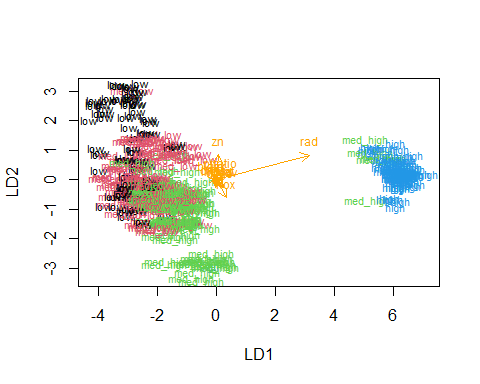
\includegraphics{chapter1_files/figure-latex/unnamed-chunk-24-1.pdf}

\hypertarget{extra-1}{%
\section{\texorpdfstring{\emph{Extra 1 }}{Extra 1 }}\label{extra-1}}

A loop to automaticlly plot histogram of all variables NB: Check that
variables are all numberical, otherwise in gender (male/female, this
will stop)

\begin{Shaded}
\begin{Highlighting}[]
\FunctionTok{colnames}\NormalTok{(learning2014[}\SpecialCharTok{{-}}\DecValTok{2}\NormalTok{]) }\CommentTok{\#[{-}2] is to remove an element of list, source: https://statisticsglobe.com/remove{-}element{-}from{-}list{-}in{-}r}
\end{Highlighting}
\end{Shaded}

\begin{verbatim}
## [1] "X"        "age"      "attitude" "deep"     "stra"     "surf"     "points"
\end{verbatim}

\begin{Shaded}
\begin{Highlighting}[]
\ControlFlowTok{for}\NormalTok{ (i }\ControlFlowTok{in} \FunctionTok{colnames}\NormalTok{(learning2014[}\SpecialCharTok{{-}}\DecValTok{2}\NormalTok{]))\{}
  \FunctionTok{print}\NormalTok{(i)}
  \FunctionTok{hist}\NormalTok{(learning2014[[i]], }\AttributeTok{col=}\StringTok{\textquotesingle{}grey\textquotesingle{}}\NormalTok{)}
\NormalTok{\}}
\end{Highlighting}
\end{Shaded}

\begin{verbatim}
## [1] "X"
\end{verbatim}

\includegraphics{chapter1_files/figure-latex/unnamed-chunk-25-1.pdf}

\begin{verbatim}
## [1] "age"
\end{verbatim}

\includegraphics{chapter1_files/figure-latex/unnamed-chunk-25-2.pdf}

\begin{verbatim}
## [1] "attitude"
\end{verbatim}

\includegraphics{chapter1_files/figure-latex/unnamed-chunk-25-3.pdf}

\begin{verbatim}
## [1] "deep"
\end{verbatim}

\includegraphics{chapter1_files/figure-latex/unnamed-chunk-25-4.pdf}

\begin{verbatim}
## [1] "stra"
\end{verbatim}

\includegraphics{chapter1_files/figure-latex/unnamed-chunk-25-5.pdf}

\begin{verbatim}
## [1] "surf"
\end{verbatim}

\includegraphics{chapter1_files/figure-latex/unnamed-chunk-25-6.pdf}

\begin{verbatim}
## [1] "points"
\end{verbatim}

\includegraphics{chapter1_files/figure-latex/unnamed-chunk-25-7.pdf}

** Visualize with ggplot**

\begin{Shaded}
\begin{Highlighting}[]
\CommentTok{\#install and load it}
\CommentTok{\#install.packages("ggplot2")}
\FunctionTok{library}\NormalTok{(ggplot2)}

\CommentTok{\# setup plot with data and aesthetic mapping}
\NormalTok{p1 }\OtherTok{\textless{}{-}} \FunctionTok{ggplot}\NormalTok{(learning2014, }\FunctionTok{aes}\NormalTok{(}\AttributeTok{x =}\NormalTok{ attitude, }\AttributeTok{y =}\NormalTok{ points, }\AttributeTok{col =}\NormalTok{ gender))}

\CommentTok{\# select visualization type (points)}
\NormalTok{p2 }\OtherTok{\textless{}{-}}\NormalTok{ p1 }\SpecialCharTok{+} \FunctionTok{geom\_point}\NormalTok{()}

\CommentTok{\# draw the plot}
\NormalTok{p2}
\end{Highlighting}
\end{Shaded}

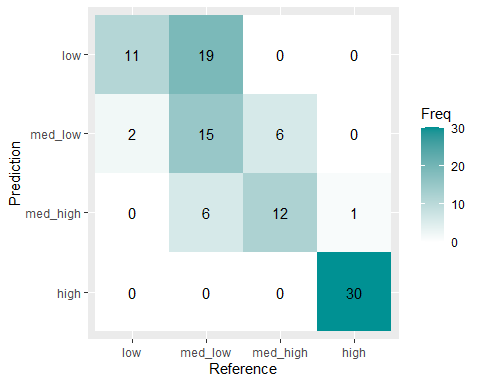
\includegraphics{chapter1_files/figure-latex/unnamed-chunk-26-1.pdf}

\begin{Shaded}
\begin{Highlighting}[]
\CommentTok{\# add a regression line}
\NormalTok{p3 }\OtherTok{\textless{}{-}}\NormalTok{ p2 }\SpecialCharTok{+} \FunctionTok{geom\_smooth}\NormalTok{(}\AttributeTok{method =} \StringTok{"lm"}\NormalTok{)}

\CommentTok{\# add a main title and draw the plot}
\NormalTok{p4 }\OtherTok{\textless{}{-}}\NormalTok{ p3 }\SpecialCharTok{+} \FunctionTok{ggtitle}\NormalTok{(}\StringTok{"Student\textquotesingle{}s attitude versus exam points"}\NormalTok{)}
\NormalTok{p4}
\end{Highlighting}
\end{Shaded}

\begin{verbatim}
## `geom_smooth()` using formula 'y ~ x'
\end{verbatim}

\includegraphics{chapter1_files/figure-latex/unnamed-chunk-27-1.pdf}

\textbf{Interpretation:}\\
As graph shows, there is a positive strong correlation between student's
attitude and their exam points the correlation was more stronger with
Male student as the slop is higher than female. So, attitude of male
student indulents the exame point more than attitue of females

\hypertarget{still-interested-on-more-visualization}{%
\subsubsection{Still interested on more
visualization?}\label{still-interested-on-more-visualization}}

If so, read this section :)\\
Draw a scatter plot matrix

\begin{Shaded}
\begin{Highlighting}[]
\CommentTok{\#pairs(learning2014[c({-}1:{-}2)])\# \_\_\_c({-}1:{-}2)\_\_\_, is to remove those column}
\FunctionTok{pairs}\NormalTok{(learning2014[}\FunctionTok{c}\NormalTok{(}\SpecialCharTok{{-}}\DecValTok{1}\SpecialCharTok{:{-}}\DecValTok{2}\NormalTok{)], }\AttributeTok{col=} \FunctionTok{c}\NormalTok{(}\StringTok{"black"}\NormalTok{,}\StringTok{"red"}\NormalTok{))}\CommentTok{\#learning2014$gender)}
\end{Highlighting}
\end{Shaded}

\includegraphics{chapter1_files/figure-latex/unnamed-chunk-28-1.pdf}
\texttt{F:\ black,\ M:\ red}

\hypertarget{do-you-wish-to-plot-even-more-fancy-and-advanced}{%
\subsubsection{Do you wish to plot even more fancy and
advanced?}\label{do-you-wish-to-plot-even-more-fancy-and-advanced}}

If yes, use GGally and ggplot2 libraries to create even more advanced
plot matrix with ggpairs()

\begin{Shaded}
\begin{Highlighting}[]
\FunctionTok{library}\NormalTok{(GGally)}
\end{Highlighting}
\end{Shaded}

\begin{verbatim}
## Registered S3 method overwritten by 'GGally':
##   method from   
##   +.gg   ggplot2
\end{verbatim}

\begin{Shaded}
\begin{Highlighting}[]
\FunctionTok{library}\NormalTok{(ggplot2)}
\NormalTok{p }\OtherTok{\textless{}{-}} \FunctionTok{ggpairs}\NormalTok{(learning2014[}\FunctionTok{c}\NormalTok{(}\SpecialCharTok{{-}}\DecValTok{1}\SpecialCharTok{:{-}}\DecValTok{2}\NormalTok{)], }\AttributeTok{mapping =} \FunctionTok{aes}\NormalTok{(), }\AttributeTok{lower =} \FunctionTok{list}\NormalTok{(}\AttributeTok{combo =} \FunctionTok{wrap}\NormalTok{(}\StringTok{"facethist"}\NormalTok{, }\AttributeTok{bins =} \DecValTok{20}\NormalTok{)))}
\NormalTok{p}
\end{Highlighting}
\end{Shaded}

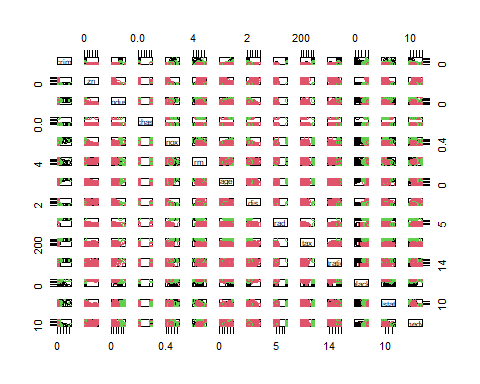
\includegraphics{chapter1_files/figure-latex/unnamed-chunk-29-1.pdf} I
hope you got facinated and liked it like me :)\\
The graph shows a (strong) negative correlation (r2= -324) between
surface and deep learning2014

\#3/////////////////\\
Now that we got familiar with variables and their distribution and
correction, it's time to fit a regression model

\hypertarget{simple-linear-regression-model}{%
\subsubsection{---- Simple linear regression model
-----}\label{simple-linear-regression-model}}

Let's create a scatter plot of points versus attitude variables

\begin{Shaded}
\begin{Highlighting}[]
\FunctionTok{qplot}\NormalTok{(attitude, points, }\AttributeTok{data =}\NormalTok{ learning2014) }\SpecialCharTok{+} \FunctionTok{geom\_smooth}\NormalTok{(}\AttributeTok{method =} \StringTok{"lm"}\NormalTok{)}
\end{Highlighting}
\end{Shaded}

\begin{verbatim}
## `geom_smooth()` using formula 'y ~ x'
\end{verbatim}

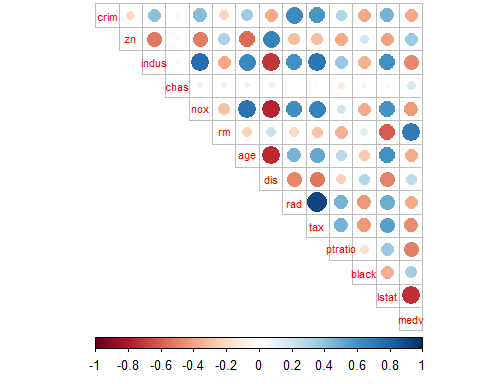
\includegraphics{chapter1_files/figure-latex/unnamed-chunk-30-1.pdf}

\begin{Shaded}
\begin{Highlighting}[]
\CommentTok{\# let\textquotesingle{}s make a simple linear regression model between exam points and attitude variables}
\NormalTok{my\_model }\OtherTok{\textless{}{-}} \FunctionTok{lm}\NormalTok{(points }\SpecialCharTok{\textasciitilde{}}\NormalTok{ attitude, }\AttributeTok{data =}\NormalTok{ learning2014)}

\CommentTok{\# print out a summary of the model}
\FunctionTok{summary}\NormalTok{(my\_model)}
\end{Highlighting}
\end{Shaded}

\begin{verbatim}
## 
## Call:
## lm(formula = points ~ attitude, data = learning2014)
## 
## Residuals:
##      Min       1Q   Median       3Q      Max 
## -16.9763  -3.2119   0.4339   4.1534  10.6645 
## 
## Coefficients:
##             Estimate Std. Error t value Pr(>|t|)    
## (Intercept)  11.6372     1.8303   6.358 1.95e-09 ***
## attitude      3.5255     0.5674   6.214 4.12e-09 ***
## ---
## Signif. codes:  0 '***' 0.001 '**' 0.01 '*' 0.05 '.' 0.1 ' ' 1
## 
## Residual standard error: 5.32 on 164 degrees of freedom
## Multiple R-squared:  0.1906, Adjusted R-squared:  0.1856 
## F-statistic: 38.61 on 1 and 164 DF,  p-value: 4.119e-09
\end{verbatim}

\textbf{Interpretation:} This model shows that attitude has
statistically significant relationship with the target variable, and can
be used to predict the exam points, becuase
Pr(\textgreater\textbar t\textbar) values are way below 0.05, thus, our
model is statistically significant in the significance level of 95\%, in
fact, this case is even valid in the significance level of
\textgreater99\%, as the values are \textless0.01" Our model will be in
fact this: \texttt{points\ =\ 3.5255*attitude+11.6372}, as linear model
is \texttt{y=ax+b}, where a is coeffient of the variable x, and b is the
intercept, both can be derive from model summary"

\hypertarget{multilinear-regression-model-with-multiple-variables--}{%
\subsubsection{---- Multilinear regression model (with multiple
variables)
----}\label{multilinear-regression-model-with-multiple-variables--}}

Let's select variables f interest and plo them:

\begin{Shaded}
\begin{Highlighting}[]
\FunctionTok{ggpairs}\NormalTok{(learning2014, }\AttributeTok{lower =} \FunctionTok{list}\NormalTok{(}\AttributeTok{combo =} \FunctionTok{wrap}\NormalTok{(}\StringTok{"facethist"}\NormalTok{, }\AttributeTok{bins =} \DecValTok{20}\NormalTok{)))}
\end{Highlighting}
\end{Shaded}

\includegraphics{chapter1_files/figure-latex/unnamed-chunk-32-1.pdf}

\begin{Shaded}
\begin{Highlighting}[]
\CommentTok{\# create a regression model with multiple explanatory variables}
\NormalTok{my\_model2 }\OtherTok{\textless{}{-}} \FunctionTok{lm}\NormalTok{(points }\SpecialCharTok{\textasciitilde{}}\NormalTok{ attitude }\SpecialCharTok{+}\NormalTok{ stra }\SpecialCharTok{+}\NormalTok{ surf, }\AttributeTok{data =}\NormalTok{ learning2014)}

\CommentTok{\# print out a summary of the model}
\FunctionTok{summary}\NormalTok{(my\_model2)}
\end{Highlighting}
\end{Shaded}

\begin{verbatim}
## 
## Call:
## lm(formula = points ~ attitude + stra + surf, data = learning2014)
## 
## Residuals:
##      Min       1Q   Median       3Q      Max 
## -17.1550  -3.4346   0.5156   3.6401  10.8952 
## 
## Coefficients:
##             Estimate Std. Error t value Pr(>|t|)    
## (Intercept)  11.0171     3.6837   2.991  0.00322 ** 
## attitude      3.3952     0.5741   5.913 1.93e-08 ***
## stra          0.8531     0.5416   1.575  0.11716    
## surf         -0.5861     0.8014  -0.731  0.46563    
## ---
## Signif. codes:  0 '***' 0.001 '**' 0.01 '*' 0.05 '.' 0.1 ' ' 1
## 
## Residual standard error: 5.296 on 162 degrees of freedom
## Multiple R-squared:  0.2074, Adjusted R-squared:  0.1927 
## F-statistic: 14.13 on 3 and 162 DF,  p-value: 3.156e-08
\end{verbatim}

In this model now, we tried to predict the exam point using attitude,
stra, and surf variables, but as the results show. only attitude has
statistically significant relation with the exam model, thus, we shall
change the other variables

\#4 /////////////////\\
It seems that there is not significant relationship between exam point
and stratigic learnign and surface. So we shall rmeove them

Lets try another model

\begin{Shaded}
\begin{Highlighting}[]
\NormalTok{my\_model3 }\OtherTok{\textless{}{-}} \FunctionTok{lm}\NormalTok{(points }\SpecialCharTok{\textasciitilde{}}\NormalTok{ attitude }\SpecialCharTok{+}\NormalTok{ stra}\SpecialCharTok{+}\NormalTok{ deep }\SpecialCharTok{+}\NormalTok{age, }\AttributeTok{data =}\NormalTok{ learning2014)}
\FunctionTok{summary}\NormalTok{(my\_model3)}
\end{Highlighting}
\end{Shaded}

\begin{verbatim}
## 
## Call:
## lm(formula = points ~ attitude + stra + deep + age, data = learning2014)
## 
## Residuals:
##      Min       1Q   Median       3Q      Max 
## -17.9941  -3.0839   0.5037   3.5519  11.3298 
## 
## Coefficients:
##             Estimate Std. Error t value Pr(>|t|)    
## (Intercept) 13.24374    3.57079   3.709 0.000286 ***
## attitude     3.53884    0.56538   6.259 3.37e-09 ***
## stra         1.05032    0.53652   1.958 0.051998 .  
## deep        -0.73226    0.74677  -0.981 0.328273    
## age         -0.08750    0.05303  -1.650 0.100866    
## ---
## Signif. codes:  0 '***' 0.001 '**' 0.01 '*' 0.05 '.' 0.1 ' ' 1
## 
## Residual standard error: 5.261 on 161 degrees of freedom
## Multiple R-squared:  0.2228, Adjusted R-squared:  0.2035 
## F-statistic: 11.54 on 4 and 161 DF,  p-value: 2.915e-08
\end{verbatim}

As model summary shows, still other variables such as age, deep, stra
are not significant, but stra is very close to significance level of
95\%, as it is Pr(\textgreater\textbar t\textbar) value is just a bit
higher than 0.05 (so, very close

\#5 /////////////////

\hypertarget{yet-another-multiple-linear-regression-model}{%
\subparagraph{Yet another multiple linear regression
model}\label{yet-another-multiple-linear-regression-model}}

\begin{Shaded}
\begin{Highlighting}[]
\NormalTok{my\_model4 }\OtherTok{\textless{}{-}} \FunctionTok{lm}\NormalTok{(points }\SpecialCharTok{\textasciitilde{}}\NormalTok{ attitude }\SpecialCharTok{+}\NormalTok{ stra, }\AttributeTok{data =}\NormalTok{ learning2014)}
\FunctionTok{summary}\NormalTok{(my\_model4)}
\end{Highlighting}
\end{Shaded}

\begin{verbatim}
## 
## Call:
## lm(formula = points ~ attitude + stra, data = learning2014)
## 
## Residuals:
##      Min       1Q   Median       3Q      Max 
## -17.6436  -3.3113   0.5575   3.7928  10.9295 
## 
## Coefficients:
##             Estimate Std. Error t value Pr(>|t|)    
## (Intercept)   8.9729     2.3959   3.745  0.00025 ***
## attitude      3.4658     0.5652   6.132 6.31e-09 ***
## stra          0.9137     0.5345   1.709  0.08927 .  
## ---
## Signif. codes:  0 '***' 0.001 '**' 0.01 '*' 0.05 '.' 0.1 ' ' 1
## 
## Residual standard error: 5.289 on 163 degrees of freedom
## Multiple R-squared:  0.2048, Adjusted R-squared:  0.1951 
## F-statistic: 20.99 on 2 and 163 DF,  p-value: 7.734e-09
\end{verbatim}

\textbf{Interpretation}\\
Same conclusion as above, stra is not statistically significant (within
significance level of 95\%), so we could either remove it from equation
(preffered), or keep it for the purpose of this practical, to have
multi-variable regression.

\begin{Shaded}
\begin{Highlighting}[]
\CommentTok{\# draw diagnostic plots using the plot() function. Choose the plots 1, 2 and 5}
\FunctionTok{par}\NormalTok{(}\AttributeTok{mfrow =} \FunctionTok{c}\NormalTok{(}\DecValTok{2}\NormalTok{,}\DecValTok{2}\NormalTok{)) }\CommentTok{\#defines that plots go to 2*2 frame (joining plots together)}
\FunctionTok{plot}\NormalTok{(my\_model4, }\AttributeTok{which =} \FunctionTok{c}\NormalTok{(}\DecValTok{1}\NormalTok{,}\DecValTok{2}\NormalTok{,}\DecValTok{5}\NormalTok{))}
\end{Highlighting}
\end{Shaded}

\includegraphics{chapter1_files/figure-latex/unnamed-chunk-36-1.pdf}
\textbf{Interpretation}\\
In linear regression, we assume:\\
1. linear relationship between variables and target variable\\
2. error are distributed normally\\
3. Errors do not correlated\\
4. errors have constant variance\\
5. the size of given error does not depend of the explanatory variables.

So, we can still check them as following:\\
To explore the normality assumption, QQ-plot can help us. As it shows,
there is a reasonable fit between the dots and the line. Thus, it was
normally distrbuted.\\
To analyse the assumption of constant variance of errors (\#4 above), we
can check residuals vs fitted plot. It shows a reasonable random
spead/distribution of dots around the line. So, this assumtion was also
valid.\\
In other words, Residual vs Fitted plot confirm that the fitted model is
appropriate becuase the variabilty of residual is not increasing with
increase of fitted value.

Residuals vs Leverage plot helps identify which observation have an
unusual high impact, like outlier. It seems that there is no such
outlier in this data

\emph{more info about interpretations:
\url{https://vimeo.com/199820384}}

\hypertarget{extra-2}{%
\subsubsection{Extra 2:}\label{extra-2}}

Let's also check the residuales of the model using a boxplot. The closer
to 0 the better the model. In other words, it shows the symmetry and
specifically the normality of the error terms in the regression model.

\begin{Shaded}
\begin{Highlighting}[]
\FunctionTok{boxplot}\NormalTok{(my\_model4}\SpecialCharTok{$}\NormalTok{residuals,}
        \AttributeTok{main =} \StringTok{"Residuals of the model"}\NormalTok{,}
        \AttributeTok{xlab =} \StringTok{"Residual values"}\NormalTok{,}
        \AttributeTok{ylab =} \StringTok{""}\NormalTok{,}
        \AttributeTok{col =} \StringTok{"orange"}\NormalTok{,}
        \AttributeTok{border =} \StringTok{"brown"}\NormalTok{,}
        \AttributeTok{horizontal =}\NormalTok{ F,}
        \AttributeTok{notch =}\NormalTok{ F)}
\end{Highlighting}
\end{Shaded}

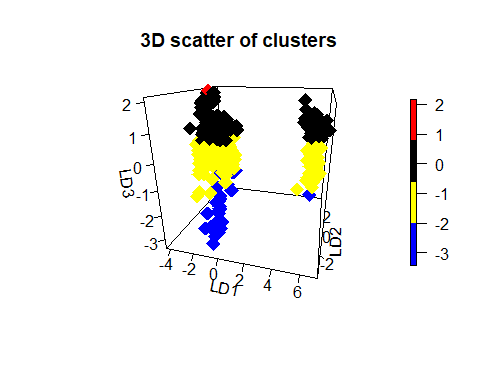
\includegraphics{chapter1_files/figure-latex/unnamed-chunk-37-1.pdf}

\hypertarget{end-of-exercise-2-linear-regression-analysis}{%
\section{END of exercise 2: linear regression
analysis}\label{end-of-exercise-2-linear-regression-analysis}}

\textbf{thank you and all the best}

\end{document}
